% !Mode:: "TeX:UTF-8"

\def\usewhat{pdflatex}                               % 定义编译方式 dvipdfmx 或者 pdflatex,默认为 dvipdfmx
                                                     % 方式编译,如果需要修改,只需改变花括号中的内容即可。
\documentclass[12pt,openany,oneside,ctexartutf8]{book}
                                                     % 本科生毕业论文通常采用单页排版
% !Mode:: "TeX:UTF-8"
%  Authors: 张井   Jing Zhang: prayever@gmail.com     天津大学2010级管理与经济学部信息管理与信息系统专业硕士生
%           余蓝涛 Lantao Yu: lantaoyu1991@gmail.com  天津大学2008级精密仪器与光电子工程学院测控技术与仪器专业本科生

%%%%%%%%%% Package %%%%%%%%%%%%
\usepackage{graphicx}                       % 支持插图处理
% \usepackage[a4paper,text={146.4true mm,239.2 true mm},top= 25.4true mm, bottom= 25.4true mm, left=31.7 true mm,head=6true mm,headsep=6.5true mm,foot=16.5true mm]{geometry}
\usepackage[a4paper,top=25.4mm, bottom=25.4mm, left=31.7mm, right=31.7mm, head=6true mm,headsep=6.5true mm,foot=17.5mm]{geometry}
                                            % 支持版面尺寸设置
\usepackage[squaren]{SIunits}               % 支持国际标准单位

\usepackage{titlesec}                       % 控制标题的宏包
\usepackage{titletoc}                       % 控制目录的宏包
\usepackage{fancyhdr}                       % fancyhdr宏包 支持页眉和页脚的相关定义
\usepackage[UTF8]{ctex}                     % 支持中文显示
\usepackage{CJKpunct}
\usepackage{color}                          % 支持彩色
\usepackage{amsmath}                        % AMSLaTeX宏包 用来排出更加漂亮的公式
\usepackage{amssymb}                        % 数学符号生成命令
\usepackage[below]{placeins}    %允许上一个section的浮动图形出现在下一个section的开始部分,还提供\FloatBarrier命令,使所有未处理的浮动图形立即被处理
\usepackage{multirow}                       % 使用Multirow宏包,使得表格可以合并多个row格
\usepackage{booktabs}                       % 表格,横的粗线;\specialrule{1pt}{0pt}{0pt}
\usepackage{longtable}                      % 支持跨页的表格。
\usepackage{tabularx}                       % 自动设置表格的列宽
\usepackage{subfigure}                      % 支持子图 %centerlast 设置最后一行是否居中
\usepackage[subfigure]{ccaption}            % 支持子图的中文标题
\usepackage[sort&compress,numbers]{natbib}  % 支持引用缩写的宏包
\usepackage{enumitem}                       % 使用enumitem宏包,改变列表项的格式
\usepackage{calc}                           % 长度可以用+ - * / 进行计算
\usepackage{txfonts}                        % 字体宏包
\usepackage{bm}                             % 处理数学公式中的黑斜体的宏包
\usepackage[amsmath,thmmarks,hyperref]{ntheorem}  % 定理类环境宏包,其中 amsmath 选项用来兼容 AMS LaTeX 的宏包
\usepackage{CJKnumb}                        % 提供将阿拉伯数字转换成中文数字的命令
\usepackage{indentfirst}                    % 首行缩进宏包
\usepackage{CJKutf8}                        % 用在UTF8编码环境下,它可以自动调用CJK,同时针对UTF8编码作了设置

% \usepackage{fancybox} 

%\usepackage{hypbmsec}                      % 用来控制书签中标题显示内容
\newcommand{\tabincell}[2]{\begin{tabular}{@{}#1@{}}#2\end{tabular}}
\usepackage{xcolor}
%支持代码环境
\usepackage{listings}
\lstset{numbers=left,
language=[ANSI]{C},
numberstyle=\tiny,
extendedchars=false,
showstringspaces=false,
breakatwhitespace=false,
breaklines=true,
captionpos=b,
keywordstyle=\color{blue!70},
commentstyle=\color{red!50!green!50!blue!50},
frame=shadowbox,
rulesepcolor=\color{red!20!green!20!blue!20}
}
%支持算法环境
\usepackage[boxed,ruled,lined]{algorithm2e}
\usepackage{algorithmic}

\usepackage{array}
\newcommand{\PreserveBackslash}[1]{\let\temp=\\#1\let\\=\temp}
\newcolumntype{C}[1]{>{\PreserveBackslash\centering}p{#1}}
\newcolumntype{R}[1]{>{\PreserveBackslash\raggedleft}p{#1}}
\newcolumntype{L}[1]{>{\PreserveBackslash\raggedright}p{#1}}

% 生成有书签的 pdf 及其生成方式。通常可以在 tjumain.tex 文件的第一行选择 pdflatex 或者是 dvipdfmx 编译手段。如果选择前者,则使用 pdflatex + pdflatex 编译; 如果选择后者,在编译的时候选择 latex + bibtex + latex + latex 编译。出现混淆的时候,系统会报错。
% 如果您的pdf制作中文书签有乱码使用如下命令,就可以解决了
\def\atemp{pdflatex}\ifx\atemp\usewhat
\usepackage{cmap}                           % pdflatex 编译时,可以生成可复制、粘贴的中文 PDF 文档, 缺点是在Windows上显示时效果不大好,字体发虚
\usepackage{hyperref}
\hypersetup{
    unicode,
    pdfborder={0 0 0},
}
\fi
% \usepackage[pdftex,unicode,
%             CJKbookmarks=true,
%             bookmarksnumbered=true,
%             bookmarksopen=true,
%             colorlinks=false,
%             pdfborder={0 0 0},
%             citecolor=blue,
%             linkcolor=red,
%             anchorcolor=green,
%             urlcolor=blue,
%             breaklinks=true
%             ]{hyperref}

                                % 定义本文所使用宏包
\graphicspath{{figures/}}                            % 定义所有的 .eps 文件在 figures 子目录下
\begin{document}                                     % 开始全文
\begin{CJK*}{UTF8}{song}                             % 开始中文字体使用
    % !Mode:: "TeX:UTF-8"
%  Authors: 张井   Jing Zhang: prayever@gmail.com     天津大学2010级管理与经济学部信息管理与信息系统专业硕士生
%           余蓝涛 Lantao Yu: lantaoyu1991@gmail.com  天津大学2008级精密仪器与光电子工程学院测控技术与仪器专业本科生

% 2018/5/23修正
%           李幼萌 Youmeng Li: liyoumeng@tju.edu.cn   天津大学软件学院软件工程系

%%%%%%%%%%%%%%%%% Fonts Definition and Basics %%%%%%%%%%%%%%%%%
\newcommand{\song}{\CJKfamily{song}}    % 宋体
\newcommand{\fs}{\CJKfamily{fs}}        % 仿宋体
\newcommand{\kai}{\CJKfamily{kai}}      % 楷体
\newcommand{\hei}{\CJKfamily{hei}}      % 黑体
\newcommand{\li}{\CJKfamily{li}}        % 隶书
\newcommand{\yihao}{\fontsize{26pt}{26pt}\selectfont}       % 一号, 单倍行距
\newcommand{\xiaoyi}{\fontsize{24pt}{24pt}\selectfont}      % 小一, 单倍行距
\newcommand{\erhao}{\fontsize{22pt}{1.25\baselineskip}\selectfont}       % 二号, 1.25倍行距
\newcommand{\xiaoer}{\fontsize{18pt}{18pt}\selectfont}      % 小二, 单倍行距
\newcommand{\sanhao}{\fontsize{16pt}{16pt}\selectfont}      % 三号, 单倍行距
\newcommand{\xiaosan}{\fontsize{15pt}{15pt}\selectfont}     % 小三, 单倍行距
\newcommand{\sihao}{\fontsize{14pt}{14pt}\selectfont}       % 四号, 单倍行距
\newcommand{\xiaosi}{\fontsize{12pt}{12pt}\selectfont}      % 小四, 单倍行距
\newcommand{\wuhao}{\fontsize{10.5pt}{10.5pt}\selectfont}   % 五号, 单倍行距
\newcommand{\xiaowu}{\fontsize{9pt}{9pt}\selectfont}        % 小五, 单倍行距

\CJKtilde  % 重新定义了波浪符~的意义
\newcommand\prechaptername{第}
\newcommand\postchaptername{章}

\punctstyle{hangmobanjiao}             % 调整中文字符的表示,行内占一个字符宽度,行尾占半个字符宽度

% 调整罗列环境的布局
\setitemize{leftmargin=3em,itemsep=0em,partopsep=0em,parsep=0em,topsep=-0em}
\setenumerate{leftmargin=3em,itemsep=0em,partopsep=0em,parsep=0em,topsep=0em}

% 避免宏包 hyperref 和 arydshln 不兼容带来的目录链接失效的问题。
\def\temp{\relax}
\let\temp\addcontentsline
\gdef\addcontentsline{\phantomsection\temp}

% 自定义项目列表标签及格式 \begin{publist} 列表项 \end{publist}
\newcounter{pubctr} %自定义新计数器
\newenvironment{publist}{%%%%%定义新环境
  \begin{list}{[\arabic{pubctr}]} %%标签格式
    {
      \usecounter{pubctr}
      \setlength{\leftmargin}{2.5em}   % 左边界 \leftmargin =\itemindent + \labelwidth + \labelsep
      \setlength{\itemindent}{0em}     % 标号缩进量
      \setlength{\labelsep}{1em}       % 标号和列表项之间的距离,默认0.5em
      \setlength{\rightmargin}{0em}    % 右边界
      \setlength{\topsep}{0ex}         % 列表到上下文的垂直距离
      \setlength{\parsep}{0ex}         % 段落间距
      \setlength{\itemsep}{0ex}        % 标签间距
      \setlength{\listparindent}{0pt}  % 段落缩进量
    }}
    {\end{list}}

\makeatletter
\renewcommand\normalsize{
  \@setfontsize\normalsize{12pt}{12pt} % 小四对应 12 pt
  \setlength\abovedisplayskip{4pt}
  \setlength\abovedisplayshortskip{4pt}
  \setlength\belowdisplayskip{\abovedisplayskip}
  \setlength\belowdisplayshortskip{\abovedisplayshortskip}
  \let\@listi\@listI}
\def\defaultfont{\renewcommand{\baselinestretch}{1.63}\normalsize\selectfont} % 设置行距

\renewcommand{\CJKglue}{\hskip -0.1 pt plus 0.08\baselineskip} % 控制字间距,使每行 34 个汉字
\makeatother

%%%%%%%%%%%%% Contents %%%%%%%%%%%%%%%%%
\renewcommand{\contentsname}{目\qquad 录}
\setcounter{tocdepth}{1} % 控制目录深度
\titlecontents{chapter}[2em]{\vspace{.5\baselineskip}\xiaosan\song}
{\prechaptername\CJKnumber{\thecontentslabel}\postchaptername\qquad}{}
{\hspace{.5em}\titlerule*[10pt]{$\cdot$}\sihao\contentspage}
\titlecontents{section}[4.2em]{\vspace{.25\baselineskip}\sihao\song}
{\thecontentslabel\quad}{}
{\hspace{.5em}\titlerule*[10pt]{$\cdot$}\sihao\contentspage}
% \titlecontents{subsection}[4em]{\vspace{.25\baselineskip}\xiaosi\song}
%              {\thecontentslabel\quad}{}
%              {\hspace{.5em}\titlerule*[10pt]{$\cdot$}\sihao\contentspage}

%%%%%%%%%% Chapter and Section %%%%%%%%%%%%%
\setcounter{secnumdepth}{4}
\setlength{\parindent}{2em}

\renewcommand{\chaptername}{\prechaptername\CJKnumber{\thechapter}\postchaptername}
\titleformat{\chapter}{\centering}{\xiaosan\song}{\chaptername}{} %{2em}
\titlespacing{\chapter}{0pt}{0.1\baselineskip}{0.8\baselineskip}

\titleformat{\section}{\sihao\hei}{\thesection}{1em}{}
\titlespacing{\section}{0pt}{0.15\baselineskip}{0.25\baselineskip}

\titleformat{\subsection}{\sihao\hei}{\thesubsection}{1em}{}
\titlespacing{\subsection}{0pt}{0.1\baselineskip}{0.3\baselineskip}

\titleformat{\subsubsection}{\sihao\hei}{\thesubsubsection}{1em}{}
\titlespacing{\subsubsection}{0pt}{0.05\baselineskip}{0.1\baselineskip}

%%%%%%%%%% Table, Figure and Equation %%%%%%%%%%%%%%%%%
\renewcommand{\tablename}{表}                                     % 插表题头
\renewcommand{\figurename}{图}                                    % 插图题头
\renewcommand{\thefigure}{\arabic{chapter}-\arabic{figure}}       % 使图编号为 7-1 的格式 %\protect{~}
\renewcommand{\thesubfigure}{\alph{subfigure})}                   % 使子图编号为 a) 的格式
\renewcommand{\thesubtable}{(\alph{subtable})}                    % 使子表编号为 (a) 的格式
\renewcommand{\thetable}{\arabic{chapter}-\arabic{table}}         % 使表编号为 7-1 的格式
\renewcommand{\theequation}{\arabic{chapter}-\arabic{equation}}   % 使公式编号为 7-1 的格式

%%%%%% 定制浮动图形和表格标题样式 %%%%%%
\makeatletter
\long\def\@makecaption#1#2{
  \vskip\abovecaptionskip
  \sbox\@tempboxa{\centering\wuhao\song{#1\qquad #2} }
  \ifdim \wd\@tempboxa >\hsize
    \centering\wuhao\song{#1\qquad #2} \par
  \else
    \global \@minipagefalse
    \hb@xt@\hsize{\hfil\box\@tempboxa\hfil}
  \fi
  \vskip\belowcaptionskip}
\makeatother
\captiondelim{~~~~} %用来控制longtable表头分隔符

%%%%%%%%%% Theorem Environment %%%%%%%%%%%%%%%%%
\theoremstyle{plain}
\theorembodyfont{\song\rmfamily}
\theoremheaderfont{\hei\rmfamily}
\newtheorem{theorem}{定理~}[chapter]
\newtheorem{lemma}{引理~}[chapter]
\newtheorem{axiom}{公理~}[chapter]
\newtheorem{proposition}{命题~}[chapter]
\newtheorem{prop}{性质~}[chapter]
\newtheorem{corollary}{推论~}[chapter]
\newtheorem{definition}{定义~}[chapter]
\newtheorem{conjecture}{猜想~}[chapter]
\newtheorem{example}{例~}[chapter]
\newtheorem{remark}{注~}[chapter]
%\newtheorem{algorithm}{算法~}[chapter]
\newenvironment{proof}{\noindent{\hei 证明:}}{\hfill $ \square $ \vskip 4mm}
\theoremsymbol{$\square$}

%%%%%%%%%% Page: number, header and footer  %%%%%%%%%%%%%%%%%

%\frontmatter 或 \pagenumbering{roman}
%\mainmatter 或 \pagenumbering{arabic}
\makeatletter
\renewcommand\frontmatter{\clearpage
  \@mainmatterfalse
}
\makeatother

%%%%%%%%%%%% References %%%%%%%%%%%%%%%%%
\renewcommand{\bibname}{参考文献}
% 重定义参考文献样式,来自thu
\makeatletter
\renewenvironment{thebibliography}[1]{
  \titleformat{\chapter}{\raggedright\sihao\hei}{\chaptername}{2em}{}
  \chapter*{\bibname}
  \wuhao
  \list{\@biblabel{\@arabic\c@enumiv}}
  {\renewcommand{\makelabel}[1]{##1\hfill}
    \settowidth\labelwidth{0 cm}
    \setlength{\labelsep}{0pt}
    \setlength{\itemindent}{0pt}
    \setlength{\leftmargin}{\labelwidth+\labelsep}
    \addtolength{\itemsep}{-0.7em}
    \usecounter{enumiv}
    \let\p@enumiv\@empty
    \renewcommand\theenumiv{\@arabic\c@enumiv}}
  \sloppy\frenchspacing
  \clubpenalty4000
  \@clubpenalty \clubpenalty
  \widowpenalty4000
  \interlinepenalty4000
  \sfcode`\.\@m}
{\def\@noitemerr
  {\@latex@warning{Empty `thebibliography' environment}}
  \endlist\frenchspacing}
\makeatother

\addtolength{\bibsep}{-0.5em}     % 缩小参考文献间的垂直间距
\setlength{\bibhang}{2em}         % 每个条目自第二行起缩进的距离

% 参考文献引用作为上标出现
%\newcommand{\citeup}[1]{\textsuperscript{\cite{#1}}}
\makeatletter
\def\@cite#1#2{\textsuperscript{[{#1\if@tempswa , #2\fi}]}}
\makeatother
%% 引用格式
\bibpunct{[}{]}{,}{s}{}{,}

%%%%%%%%%%%% Cover %%%%%%%%%%%%%%%%%
% 封面、摘要、版权、致谢格式定义
\makeatletter
\def\ctitle#1{\def\@ctitle{#1}}\def\@ctitle{}
\def\cdegree#1{\def\@cdegree{#1}}\def\@cdegree{}
\def\caffil#1{\def\@caffil{#1}}\def\@caffil{}
\def\csubject#1{\def\@csubject{#1}}\def\@csubject{}
\def\cgrade#1{\def\@cgrade{#1}}\def\@cgrade{}
\def\cauthor#1{\def\@cauthor{#1}}\def\@cauthor{}
\def\cnumber#1{\def\@cnumber{#1}}\def\@cnumber{}
\def\cstuid#1{\def\@cstuid{#1}}\def\@cstuid{}
\def\cdate#1{\def\@cdate{#1}}\def\@cdate{}
\long\def\cabstract#1{\long\def\@cabstract{#1}}\long\def\@cabstract{}
\long\def\eabstract#1{\long\def\@eabstract{#1}}\long\def\@eabstract{}
\def\ckeywords#1{\def\@ckeywords{#1}}\def\@ckeywords{}
\def\ekeywords#1{\def\@ekeywords{#1}}\def\@ekeywords{}
\def\cheading#1{\def\@cheading{#1}}\def\@cheading{}
\def\ccovertitle#1{\def\@ccovertitle{#1}}\def\@ccovertitle{}

\pagestyle{fancy}
\fancyhf{}
\fancyhead[C]{\song\wuhao \@cheading}  % 页眉显示天津大学 20XX 届本科生毕业论文
\fancyfoot[C]{\song\xiaowu ~\thepage~}
\newlength{\@title@width}

% 定义封面
\def\makecover{
  %\cleardoublepage%
  \phantomsection
  \pdfbookmark[-1]{\@ctitle}{ctitle}

  \begin{titlepage}
    \vspace*{10pt}
    \begin{center}

      \begin{figure}[h]
        \centering
        
\includegraphics[width=0.4\textwidth]{figures/tju}
      \end{figure}
      \vspace*{15pt}
      \hei\erhao{\textbf{\@ccovertitle}} \\
      \hei\erhao{\textbf{\@ctitle}}
      \vspace*{55pt}

      \begin{figure}[h]
        \centering
        
\includegraphics[width=0.3\textwidth]{figures/Tjulogo}
      \end{figure}

      \vspace*{60pt}
      \renewcommand\arraystretch{1.5}
      \setlength{\@title@width}{10cm}
      {
        \sanhao\song{
          \begin{tabular}{lc}
            \textbf{学\qquad 院} & \underline{\makebox[\@title@width][c]{\textbf{\@caffil}}}   \\
            \textbf{专\qquad 业} & \underline{\makebox[\@title@width][c]{\textbf{\@csubject}}} \\
            \textbf{年\qquad 级} & \underline{\makebox[\@title@width][c]{\textbf{\@cgrade}}}   \\
            \textbf{姓\qquad 名} & \underline{\makebox[\@title@width][c]{\textbf{\@cauthor}}}  \\
            \textbf{学\qquad 号} & \underline{\makebox[\@title@width][c]{\textbf{\@cstuid}}}   \\
          \end{tabular}
        }
      }
      \vspace*{40pt}

      \song\sanhao{\textbf{\@cdate}}
    \end{center}
  \end{titlepage}
}

                             % 完成对论文各个部分格式的设置
    % !Mode:: "TeX:UTF-8"


%%%%%%%%%%%%%%%%%%%%%%%%%%%%%%%%%%%%%%%%%%%%%%%%%%%%%%%%%%%%%%%
%%  可通过对 setup/format.tex中                               %%
%%  第243行 \setlength{\@title@width}{5cm}中 5cm 这个参数来   %%
%%  控制封面中下划线的长度。                                   %%
%%%%%%%%%%%%%%%%%%%%%%%%%%%%%%%%%%%%%%%%%%%%%%%%%%%%%%%%%%%%%%

\cheading{天津大学软件学院~\the\year~年 软件工程综合实践报告}      % 正文页眉
\ccovertitle{软件工程综合实践}                       % 封面标题

%%%%%%%%%%%%%%%%%%%%%%%%%%%%%%%%%%%%%%%%%%%%%%%%%%%%%%%%%%%%%
%%%%%%%%%% 以下为论文的基本信息,需要由作者进行修改 %%%%%%%%%%%%
%%%%%%%%%%%%%%%%%%%%%%%%%%%%%%%%%%%%%%%%%%%%%%%%%%%%%%%%%%%%%
\ctitle{实践报告}    % 封面用论文标题,自己可手动断行
\caffil{智能与计算学部}       % 学院名称
\csubject{软件工程}     % 专业名称
\cgrade{2020级}           % 年级
\cauthor{梁益铭、郑志嘉、周圣喻}          % 学生姓名
\cstuid{3020244108、3020244109、3020244111}     % 学号

\cdate{\the\year~年~\the\month~月~\the\day~日}  % 论文完成日期,不需要修改,自动生成

    \frontmatter                                     % 以下是论文导言部分,包括论文的封面,中英文摘要和中文目录
    \fancypagestyle{plain}{							 % 正文前均无页眉
        \fancyhf{}
        \renewcommand{\headrulewidth}{0 pt}
        \fancyfoot[C]{\song\xiaowu~\thepage~}
    }

    \makecover 			% 封面

    % !Mode:: "TeX:UTF-8"

% 目录
\defaultfont
\clearpage{
    \pagestyle{empty}
    \cleardoublepage
    \setcounter{page}{1}                                 % 单独从 1 开始编页码
    \pagenumbering{arabic}
    \titleformat{\chapter}{\centering\sanhao\hei}{\chaptername}{2em}{} % 设置目录两字的格式
    \pdfbookmark[0]{目~~录}{mulu}
    \tableofcontents                                     % 中文目录
    \thispagestyle{plain}
} % 目录

    \mainmatter\defaultfont\sloppy\raggedbottom
    \makeatletter
    \fancypagestyle{plain}{                              % 设置正文眉页脚风格
        \fancyhf{}
        \fancyhead[C]{\song\wuhao \@cheading}            % 页眉格式
        \fancyfoot[C]{\song\xiaowu ~\thepage~}           % 页脚格式
        \renewcommand{\headrulewidth}{0.5pt}
        \renewcommand{\footrulewidth}{0pt}
    }
    \makeatother
    \setcounter{page}{1}                                 % 单独从 1 开始编页码
    \titleformat{\chapter}{\centering\xiaosan\hei}{\chaptername}{2em}{} % 恢复chapter标题格式要求

    %%%%%% 这里是正文,每个文件对应正文中的一章 %%%%%%
    % !Mode:: "TeX:UTF-8"

\chapter{JDBC项目}
    % !Mode:: "TeX:UTF-8"

\chapter{前端项目}

\section{项目需求}

前端项目是第二阶段,使用HTML+CSS+JS技术开发企业级静态网页,完成后续项目中前端部分的布局。使用HTML技术完成前端静态网页应用程序的实现,使用CSS技术对网页进行样式渲染,使用JavaScript语言制作网页特效。

\subsection{首页功能}
\subsubsection*{\normalsize主要功能}
显示点餐分类信息
\subsubsection*{\normalsize动作}
1.点击点餐分类小图片,跳转到商家列表页面

2.点击下方菜单栏中的“订单”,跳转到历史订单页面

\subsection{商家列表页面功能}
\subsubsection*{\normalsize主要功能}
显示商家列表信息
\subsubsection*{\normalsize动作}
点击某个商家,跳转到此商家的详细信息页面

\subsection{商家详细信息页面功能}
\subsubsection*{\normalsize主要功能}
显示商家详细信息及所属食品信息
\subsubsection*{\normalsize动作}
点击“去结算”按钮,跳转到确认订单页面

\subsection{确认订单页面功能}
\subsubsection*{\normalsize主要功能}
1.显示订单信息

2.选择送货地址
\subsubsection*{\normalsize动作}
1.点击送货地址,跳转到送货地址列表页面

2.点击“去支付”按钮,跳转到支付页面

\subsection{在线支付页面功能}
\subsubsection*{\normalsize主要功能}
显示订单信息及订单明细信息
\subsubsection*{\normalsize动作}
无

\subsection{登录页面功能}
\subsubsection*{\normalsize主要功能}
用户登录
\subsubsection*{\normalsize动作}
1.点击“登陆”按钮,跳转到上一个页面

2.点击“去注册”按钮,跳转到注册页面

\subsection{注册页面功能}
\subsubsection*{\normalsize主要功能}
注册新用户
\subsubsection*{\normalsize动作}
点击“注册”按钮,跳转到登陆页面

\subsection{历史订单页面功能}
\subsubsection*{\normalsize主要功能}
显示用户历史订单信息
\subsubsection*{\normalsize动作}
点击某个历史订单,可以对订单明细信息进行显示和隐藏

\begin{figure}[H]
    \centering
    \subfigure{
        \begin{minipage}[t]{0.22\linewidth}
            \centering
            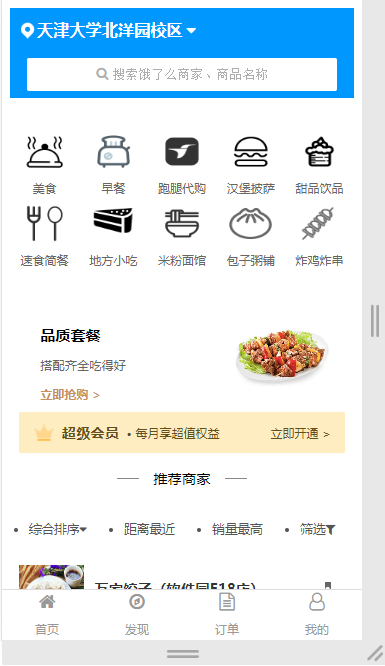
\includegraphics[scale=0.3]{figures/2.2.1.png}\\
            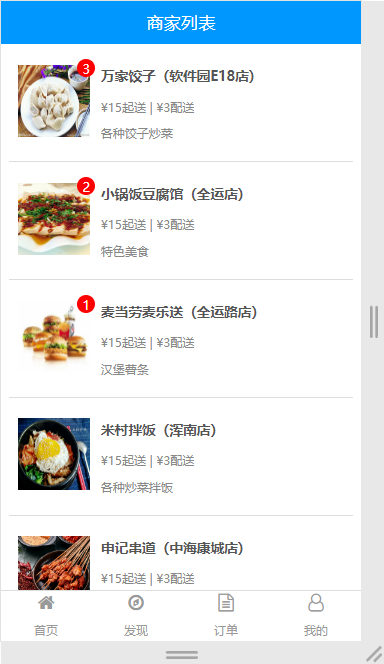
\includegraphics[scale=0.3]{figures/2.2.2.png}\\
        \end{minipage}
    }
    \subfigure{
        \begin{minipage}[t]{0.22\linewidth}
            \centering
            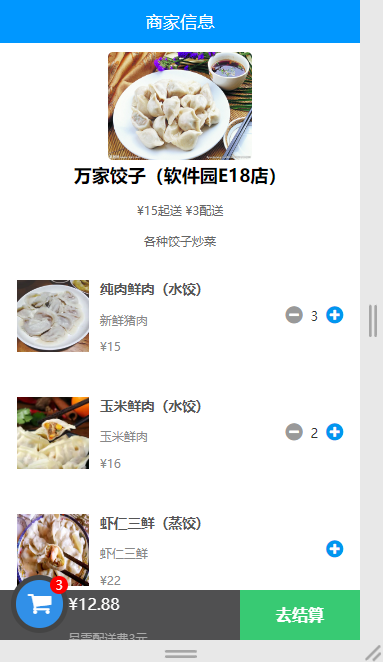
\includegraphics[scale=0.3]{figures/2.2.3.png}\\
            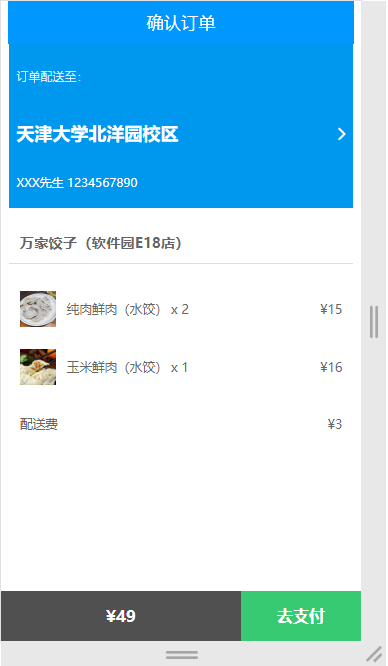
\includegraphics[scale=0.3]{figures/2.2.4.png}\\
        \end{minipage}
    }
    \subfigure{
        \begin{minipage}[t]{0.22\linewidth}
            \centering
            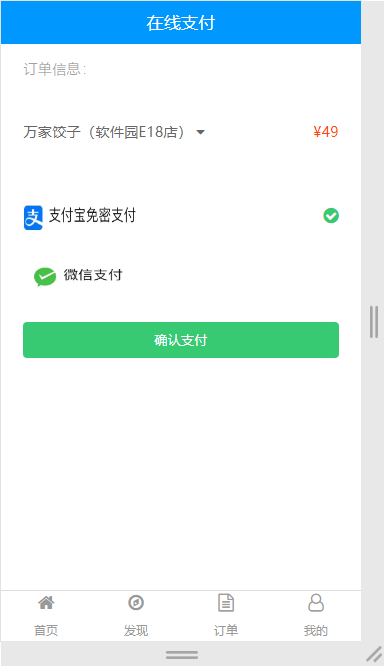
\includegraphics[scale=0.3]{figures/2.2.5.png}\\
            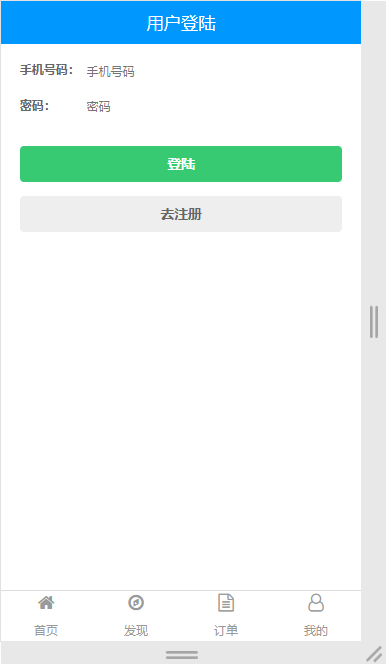
\includegraphics[scale=0.3]{figures/2.2.6.png}\\
        \end{minipage}
    }
    \subfigure{
        \begin{minipage}[t]{0.22\linewidth}
            \centering
            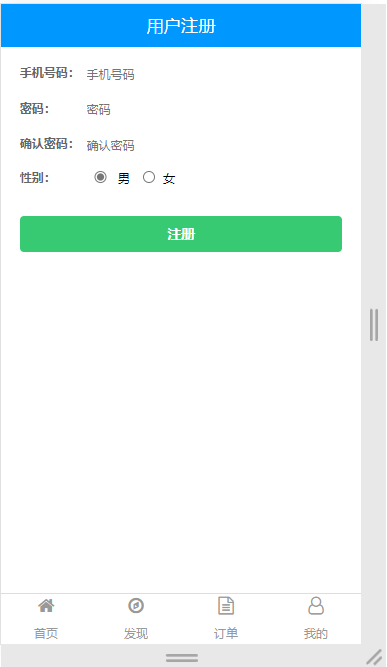
\includegraphics[scale=0.3]{figures/2.2.7.png}\\
            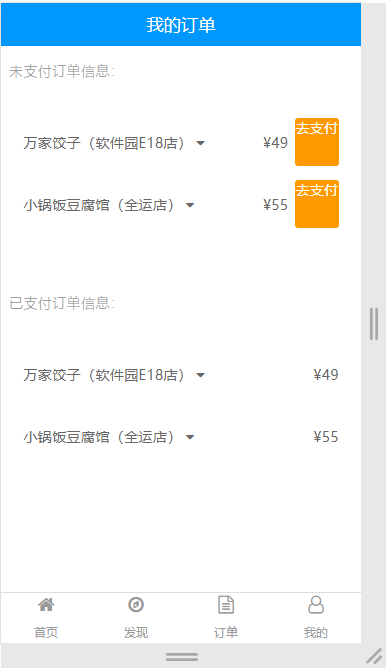
\includegraphics[scale=0.3]{figures/2.2.8.png}\\
        \end{minipage}
    }
    \centering
    \caption{前端页面实现结果}
\end{figure}

\section{项目设计}
\subsection{移动端网页设计}
\subsubsection*{\normalsize问题}
移动端屏幕尺寸多变,不像PC端屏幕那样统一。这样就造成在移动端显示网页时,由于尺寸问题,会出现显示不下
网页,从而出现横向滚动条现象。 为了解决这个问题,出现了viewport(屏幕视口)的概念。
\subsubsection*{\normalsize解决方案}
使用viewport解决上述问题。先将网页放入layout viewport中,然后在将layout viewport等比例缩小到ideal viewport中。这样就能保证:无论什么样的网页,都能在手机屏幕上显示,而且没有横向滚动条。

\subsection{弹性布局}
\subsubsection*{\normalsize概念:主轴和侧轴}
弹性布局中的一个重要概念:主轴与侧轴: 弹性盒子中默认存在两根轴,一个是水平方向的主轴,一个是垂直方向的侧轴。
\begin{figure}[H]
    \centering
    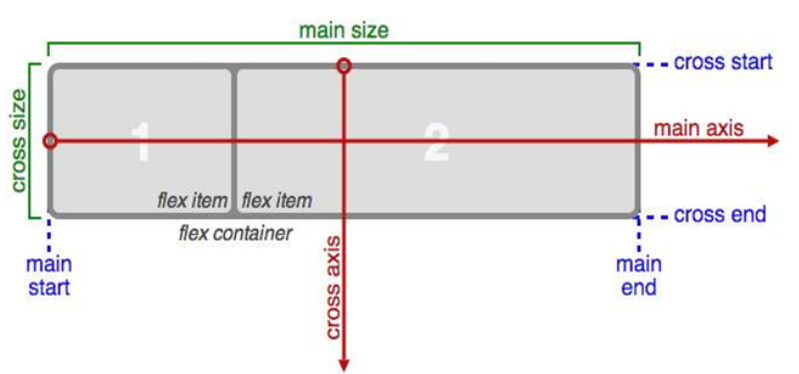
\includegraphics[scale=0.7]{figures/2.2.9.png}
    \caption{主轴和侧轴}
\end{figure}

\subsubsection*{\normalsize设计方法}
1.使用flex-direction属性设置主轴方向。

2.使用flex-wrap:wrap让子元素自动换行。

3.设置align-items样式。常用值有三种:flex-start(上对齐)、flex-end(下对齐)、center(居中)。

4.使用flex给子元素分配空间,从而让每个子元素所占空间不一致。

\subsection{视口尺寸}
视口:在PC端,指浏览器的可视区域;在移动端,指Viewport 中的 Layout Viewport。 视口尺寸常用的有以下2
个: vw : 1vw 等于视口宽度的1\% vh : 1vh 等于视口高度的1\% 实际应用中,可以使用vw,实现元素宽度和高度成
比例自动缩放。

\subsection{边框盒子模型}
CSS3之前的盒子模型,可以说是content-box型盒子,即宽和高为内容。 CSS3之后新增了一的盒子模型,可以说
是border-box型盒子,即宽和高为边框。 那么,使用box-sizing属性可以设置盒子模型类型。
    % !Mode:: "TeX:UTF-8"

\chapter{Servlet 项目}

\section{项目需求}

本项目要求使用VUE+Servlet+AJAX技术,开发前后端分离的饿了么Web应用程序。主要设计参照 “饿了么官网网页版”制作,并且仅关注点餐业务线功能,“饿了么官网”中的其它功能暂不涉及。

本项目需要完成的功能大致分为十一个页面:

1.首页:显示点餐分类信息

2. 商家列表页面:根据点餐分类显示商家列表信
息, 如果处于登录状态,那些需要
查询购物车中是否有此商家的
食品。如果有,在页面上显示
食品数量。

3.商家详细信息页面:显示商家详细信息及所属食品信
息,并自动计算总价。

4.确认订单页面:确认订单信息是否正确;选择送货地址。

5.在线支付页面:显示订单信息及订单明细信息。

6.送货地址页面:显示当前用户的送货地址信息。

7.新增送货地址页面:添加新的送货地址。

8.编辑送货地址页面:编辑送货地址。

9.登录页面:用户登录。

10.注册页面:注册新用户。

11.历史订单页面:显示用户历史订单信息。~\\


\section{项目设计}

\noindent
一. 开发环境:

1. 开发工具:IDEA、DataGrip

2. 检查IDEA的jdk配置:jdk8

3. 检查IDEA的tomcat配置:tomcat9.0.65

4. 检查IDEA的文件编码配置:utf-8

5  检查数据库配置:MySQL8.0.30~\\

\noindent
二. 数据库设计:

本项目使用MySQL数据库,选择DataGrip作为开发工具。在数据表的设计上,需要创建商家表、食品表、购物车表、送货地址表、订单表、订单明细表、用户表共七张表。

\begin{figure}[H]
    \centering
    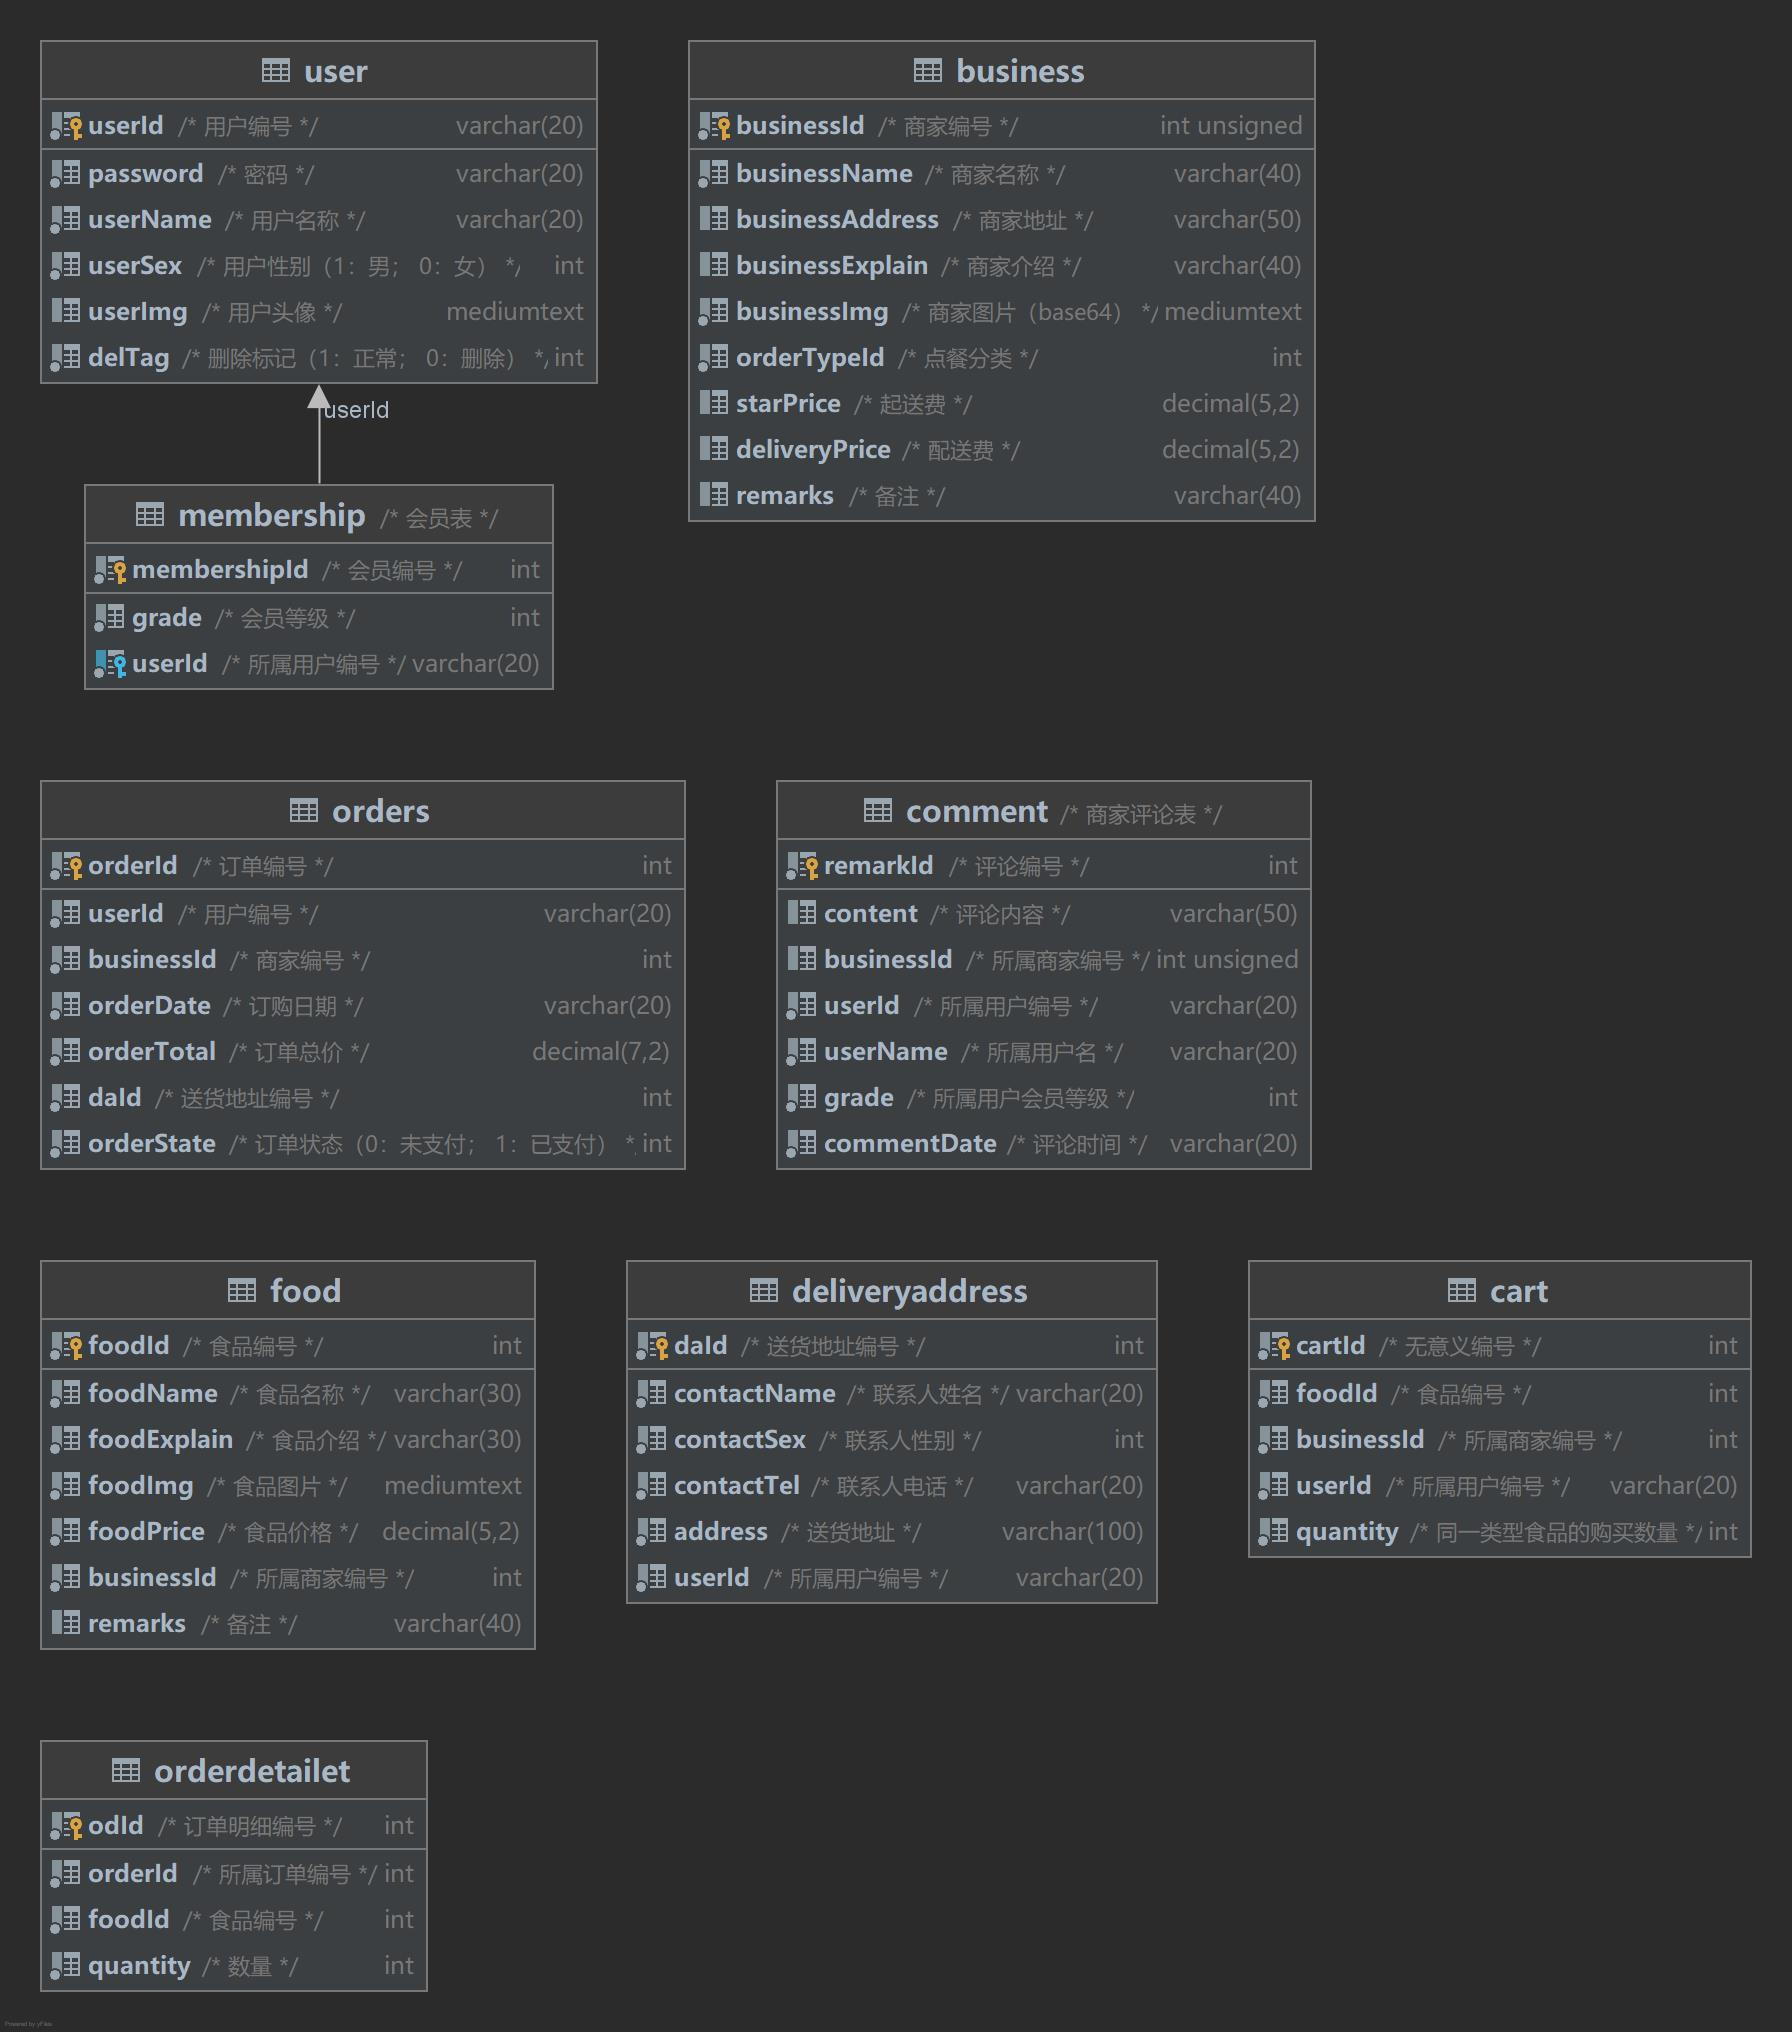
\includegraphics[width=15cm,height=17cm]{figures/table2.jpg}
    \caption{Servlet项目数据表}
    \end{figure}

\noindent
三. 服务端设计:

本项目为JavaWeb项目,在后端使用Servlet技术,Tomcat作为容器进行项目开发。在JavaWeb工程的搭建方面,本项目使用基于Servlet的简易MVC架构,能够很好地解决后端与前端地交互。在响应前端请求方面,使用Jackson将java对象或集合转换为json对象或数组后,返回前端。

\begin{figure}[H]
    \centering
    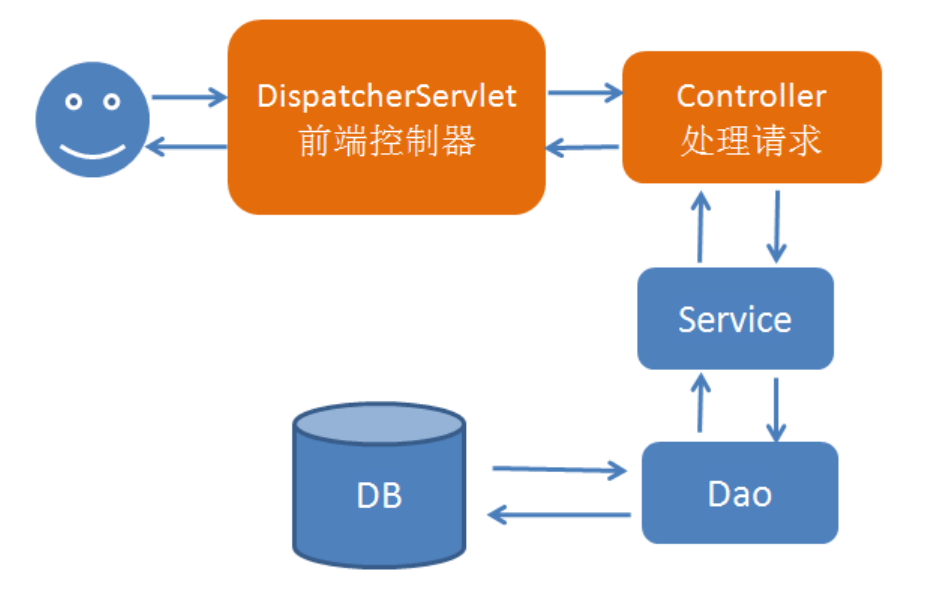
\includegraphics[width=15cm,height=10cm]{figures/MVC.png}
    \caption{Servlet简易MVC架构}
    \end{figure}

在解决




    % !Mode:: "TeX:UTF-8"

\chapter{功能创新}

在第四阶段完成后,我们意识到该项目还有许多值得改进和优化的地方,因此我们基于第四阶段的SpringBoot项目添加了一些新功能。~\\

\section{会员功能}
\subsection{功能需求}
在首页,我们发现有一个注册会员入口,而这个功能在课程中并未实现,于是我们首先选择添加一个会员功能。
用户可以选择注册成为不同等级的会员从而享受到不同程度的折扣。
用户在支付订单页面可以查看打折后的价格,点击支付以支付优惠价。~\\

\subsection{功能设计}
用户在首页可以点击“立即开通”可以进入会员注册界面,
有三种会员可以选择,分别是白银会员、黄金会员和钻石会员。
每种会员的价格不同,折扣力度也不同。
点击“去注册”可以发送注册请求。
注册请求分为3种情况:

1.如果用户不是会员,则会注册为选择的会员;

2.如果用户已经是会员且选择的会员比原本的会员等级高,则会升级会员;

3.如果用户已经是会员但选择的会员等级低于原本的会员等级,则会注册失败并返回错误信息。~\\

\subsection{数据库设计}
为了实现会员功能,需要在数据库中新增一张会员表,具体属性和与其他表的关联关系如图所示:

\begin{figure}[H]
    \centering
    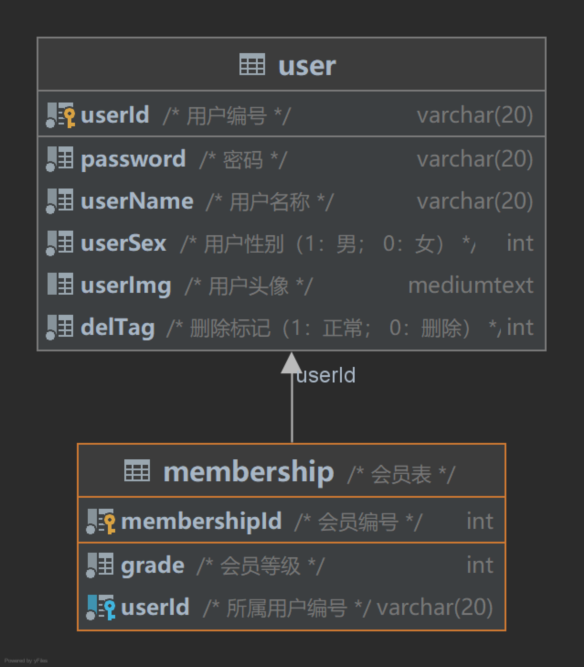
\includegraphics[width=13cm,height=15cm]{figures/table3.png}
    \caption{会员表}
\end{figure}

\subsubsection{接口文档}
1.Membership

1.1 MembershipController/getMembershipById(post方法)

参数:user

返回值:grade会员等级

功能:查询当前用户的会员等级

1.2 MembershipController/saveMembership(post方法)

参数:userId、grade

返回值:数据库改变的行数

功能:为一个用户注册会员

1.3 MembershipController/updateMembership(post方法)

参数:userId、grade

返回值:数据库改变的行数

功能:为一个用户升级会员~\\

\subsection{实现结果}
\begin{figure}[H]
    \centering
    \subfigure{
        \begin{minipage}[t]{0.48\linewidth}
            \centering
            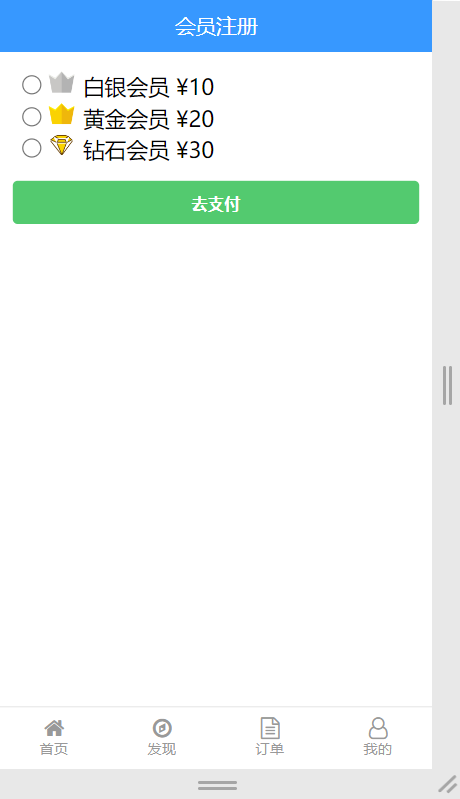
\includegraphics[scale=0.5]{figures/5.1.1.png}\\
        \end{minipage}
    }
    \subfigure{
        \begin{minipage}[t]{0.48\linewidth}
            \centering
            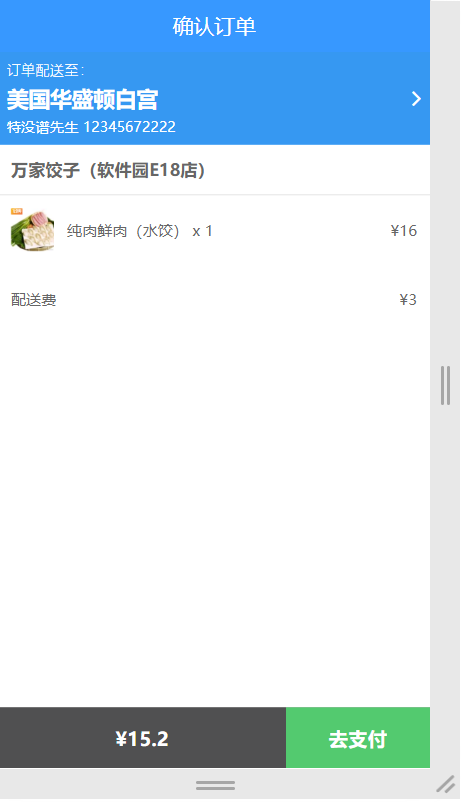
\includegraphics[scale=0.5]{figures/5.1.2.png}\\
        \end{minipage}
    }
    \centering
    \caption{会员功能实现结果}
\end{figure}

\section{“我的”页面}
\subsection{功能需求}
在网页下方的导航栏有一个“我的”按钮,在原来的实现中点击这个按钮并不会跳转到任何页面,于是我们决定实现一个“我的”页面。~\\

\subsection{功能设计}
“我的”页面最上面会显示用户姓名、ID和会员等级,若未注册会员则默认为普通会员。
在用户信息的下面,添加“我的地址”和“注册会员”按钮,分别可以路由到编辑地址和注册会员页面。~\\

\subsection{接口文档}
2.MyProfile

2.1 MembershipController/getMembershipById(post方法)

参数:user

返回值:grade会员等级

功能:查询当前用户的会员等级~\\

\subsection{实现结果}
\begin{figure}[H]
    \centering
    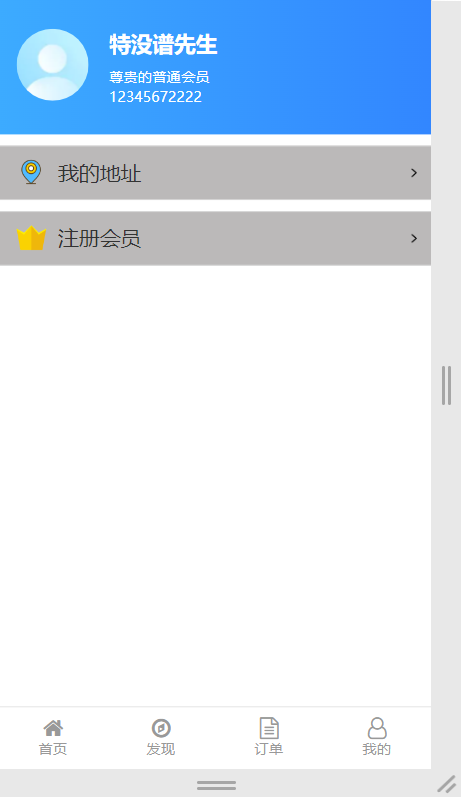
\includegraphics[scale=0.5]{figures/5.1.3.png}
    \caption{“我的”页面实现结果}
\end{figure}

\section{评论功能}
\subsection{功能需求}
在日常使用外卖APP时,我们经常会查看用户对商家的评价,
于是我们打算实现一个商家评论功能方便用户查看一个商家的评价~\\

\subsection{功能设计}
用户在支付了一个订单之后,在订单页面可以点击“去评价”,用户进入评价页面可以编写评价,点击发布即可成功发布。
点击商家信息界面中的“评价”按钮可以进入商家评价页面查看自己和其他人的评价,每条评价会显示评价人姓名、会员等级、评价时间和评价内容。~\\

\subsection{数据库设计}
为了实现评论功能,需要在数据库中添加一张评论表,具体属性和其他表的关联关系如图所示:

\begin{figure}[H]
    \centering
    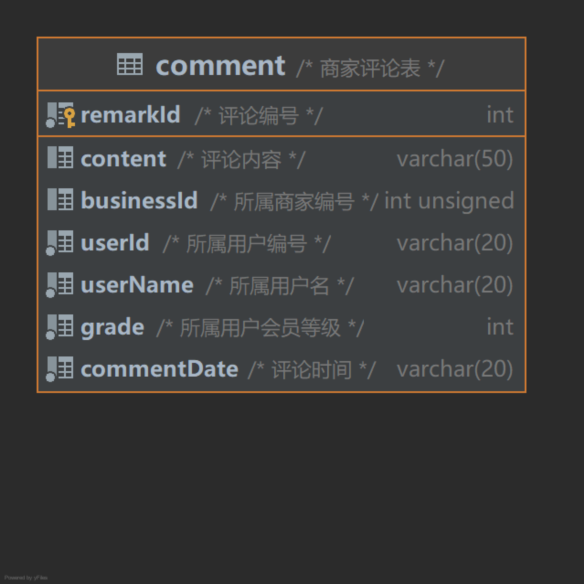
\includegraphics[width=13cm,height=13cm]{figures/table4.png}
    \caption{“我的”页面实现结果}
\end{figure}

\subsection{接口文档}
3.Comment

3.1 CommentController/listCommentByBusinessId

参数:businessId

返回值:commentArr

功能:得到评论数据库的所有内容

3.2 CommentController/saveComment

参数:userId、userName、businessId、content、grade

返回值:数据库改变的行数

功能:保存一个评论~\\

\subsection{实现结果}
\begin{figure}[H]
    \centering
    \subfigure{
        \begin{minipage}[t]{0.48\linewidth}
            \centering
            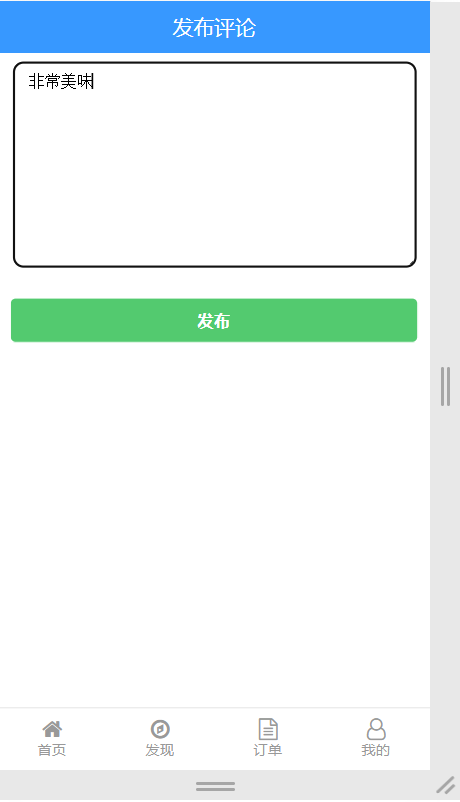
\includegraphics[scale=0.5]{figures/5.1.4.png}\\
        \end{minipage}
    }
    \subfigure{
        \begin{minipage}[t]{0.48\linewidth}
            \centering
            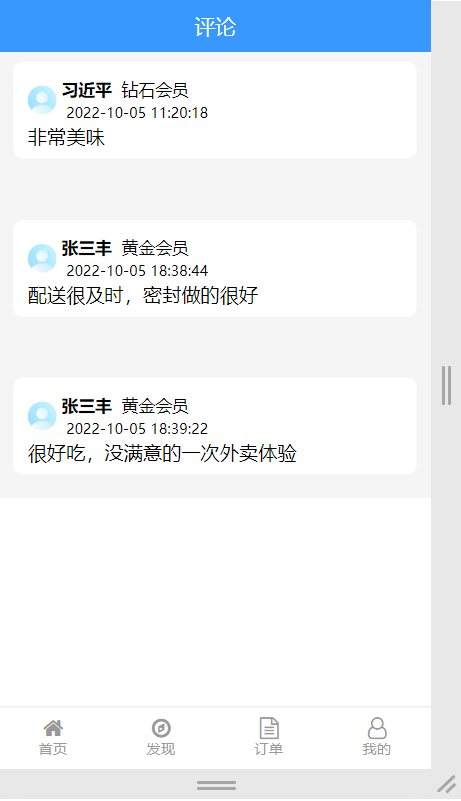
\includegraphics[scale=0.5]{figures/5.1.5.png}\\
        \end{minipage}
    }
    \centering
    \caption{评论员功能实现结果}
\end{figure}




    % \clearpage

\end{CJK*}                                     % 结束中文字体使用
\end{document}                                 % 结束全文